% SPDX-License-Identifier: GPL-2.0-or-later
% Copyright 2018 Association Prologin <info@prologin.org>

%LaTeX Document
\documentclass[a4paper,twoside,12pt]{article}
\usepackage{xltxtra}
\usepackage{url}
\usepackage{caption}
%\usepackage{lettrine}
\usepackage{amssymb}
\usepackage{wrapfig}
\usepackage{longtable}
\usepackage{booktabs}
\usepackage{hyperref}
\setromanfont[Mapping=tex-text]{TeX Gyre Pagella}
\setsansfont[Mapping=tex-text]{DejaVu Sans}
\setmonofont[
  Mapping=tex-text,
%  Scale=0.85,
  AutoFakeSlant,
  BoldItalicFeatures={FakeSlant}]{Inconsolata}
%\newfontfamily{\A}[Scale=0.85]{DejaVu Sans} % TODO find a free Arial/Helvetica equivalent
%\newfontfamily{\J}[Scale=0.85]{Hiragino Kaku Gothic Pro}
%\newfontfamily{\P}[Scale=0.85]{Palatino}
\usepackage{soul} % Pour barrer
\usepackage{textcomp} % Pour les trademarks


\usepackage{cellspace}
\setlength\cellspacetoplimit{4pt}
\setlength\cellspacebottomlimit{4pt}
\newcommand\cincludegraphics[2][]{\raisebox{-0.2\height}{\includegraphics[#1]{#2}}}

%%%%%%%%%%%%%%%%%%%%%%%%%%%%%%%%
%%         BEGIN FIXME         %
%%%%%%%%%%%%%%%%%%%%%%%%%%%%%%%%
\def\plongday{Vendredi}
\def\pday{9}
\def\pmonth{Juillet}
\def\pyear{2021}

\def\ptitle{\textsc{Panda Race}} %% Subject's main title
\def\psubtitle{Championnat Des Pandas} %% Subject's sub title

\def\plogo{logo2021.png} %% Logo FIXME
\def\psubjectpicture{logo_finale_2021.png} %% Picture to be displayed FIXME

%% on its own page \vspace*{0.1cm}}
%%%%%%%%%%%%%%%%%%%%%%%%%%%%%%%%
%%         END FIXME           %
%%%%%%%%%%%%%%%%%%%%%%%%%%%%%%%%


%%%%%%%%%%%%%%%%%%%%%%%%%%%%%%%%%%%%%%%%%%%%%%%%%%%%%%%%
%%              DO NOT EDIT PAST THIS LINE            %%
%%%%%%%%%%%%%%%%%%%%%%%%%%%%%%%%%%%%%%%%%%%%%%%%%%%%%%%%











%\documentclass[a4paper,twoside,12pt]{book}

\usepackage[french]{babel} % TODO switch to polyglossia?
\usepackage{geometry}
\usepackage{multicol}
\usepackage{fancyhdr}
\usepackage{listings}
\usepackage{array}
\usepackage{color}
\usepackage{caption}
\usepackage{subcaption}
\usepackage{amsmath}
\usepackage{tikz}

\graphicspath{{img/}}

\def\pdate{\plongday{} \pday{} \pmonth{} \pyear{}}
\def\tightlist{} % fix for pandoc

\definecolor{colIdentifier}{gray}{0}
\definecolor{colKeys}{rgb}{0,0,0.6}
\lstset{
    extendedchars=false,
    showstringspaces=false,
    escapeinside=@@,
%    keywordstyle=\color{blue},
%    commentstyle=\color[rgb]{0.133,0.545,0.133},
    columns=flexible,
    language=C++,
    tabsize=2,
    basicstyle=\ttfamily\NoAutoSpacing
%    numbers=left,
%    frame=lines
}
\lstnewenvironment{lst-c++}{%
\lstset{%
  breaklines=true,
  postbreak=\mbox{\textcolor{red}{$\hookrightarrow$}\space},
  language=C++
}}{}

\newcommand{\wfig}[2]{
}


\captionsetup{justification=centering}

%\renewcommand\ttdefault{cmtt}

\newcommand{\functitle}[1]{%
\vspace{0.5cm}
$\bullet$ \underline{\textbf{#1}}
}

%\NoAutoSpaceBeforeFDP
\geometry{bindingoffset=5mm,hmarginratio=1:1,heightrounded,headheight=15pt,bmargin=3cm}

\setcounter{tocdepth}{2}

\makeindex

\begin{document}
\pagestyle{empty}
\sloppy

\lhead[\thepage]{\nouppercase \leftmark}
\rhead[\textsl{Prologin \pyear{}} --- Sujet de la finale en ligne]{\thepage}
%%\cfoot{\color{red}TOP SECRET//SI//ORCON//NOFORN}

\sethlcolor{black}

% Couverture =========================================================
\begin{titlepage}
\begin{center}
~\includegraphics[width=\linewidth]{\plogo}\\
\vspace{5cm}
\Huge
\textbf{\ptitle{}}

\vspace{1cm}

\Large
\textbf{\psubtitle{}}

\vspace{2cm}

\normalsize
\textnormal Sujet de la finale en ligne du Concours National d'Informatique\\
\pdate\\

\end{center}


\end{titlepage}

\small

% Sommaire ===========================================================
\cleardoublepage
\tableofcontents

\normalsize

% Corps ==============================================================
%\cleardoublepage
\setcounter{page}{1}
\pagestyle{fancy}
\parskip=6pt plus 3pt

\newpage
\vspace{4cm}
\begin{center}\includegraphics[height=14cm]{\psubjectpicture}\end{center}

\pagebreak
\section{Contexte} % on peut changer "Contexte" pour aurte chose

% Bravo et Félicitations ...

\subsection{Tournoi bicentennal\protect\footnote{périodicité de 200 ans} des Pandas} %  Concours bicentennal de parentage ?

% Côté RP du concours

Comme vous le savez très certainement, la Chine est un grand pays\footnote{9,597 millions km²} regorgeant de traditions vieilles comme le monde\footnote{Nous considèrerons l'arrivée des Ailuropoda melanoleuca (Panda) comme la génèse de ce bas-monde}. L'une d'entre elles est pratiquée, encore à ce jour, par les Pandas Géants et les Pandas Roux. En effet, des observations récentes nous montrent qu'ils pratiquent un rituel, lors duquel la meilleure race de panda est reconnue pour les deux siècles à venir. Par souci d'équité et de justice, le jury n'est pas composé de pandas.
% parler plus du jury ? :thinking:

\subsection{Le championnat}
Le but du championnat est de trouver quelle race compte le meilleur couple de parents\footnote{On remarquera un grand nombre de pédiatres au sein des deux communautés pandesques}. Des bébés pandas seront disposés sur la rivière, dans le grand danger des torrents. Le but des parents est d'aller récupérer tous leurs petits. Le premier couple à avoir récupéré tous les pandas a gagné le match !\footnote{Vous jouerez en effet les deux parents, et non pas un seul panda}

\subsection{Champ de bataille}
Le champ de bataille sera cette année la rivière de \textit{Hulun}, au Nord-Ouest du pays oriental, hôte de ce championnat depuis toujours : la Chine. La rivière, à l'apparence rectangulaire est en fait composée d'hexagones, à travers lesquels des pandas de toutes sortes\footnote{Vous et vos adversaires} devront se mouvoir.

\newpage

\subsubsection{Eau}
L'eau est surprenamment l'élément le plus présent dans la rivière. Il est le premier obstacle. Les pandas ne peuvent pas aller sur l'eau. Ils doivent marcher sur les ponts. Les bébés pandas se trouvent uniquement sur des cases d'eau.

\begin{center}
    
\includegraphics[width=3cm]{water_example.png}
\end{center}

\subsubsection{Ponts}
Les ponts sont le seul moyen de déplacement des pandas. Les ponts sont constitués de deux cases distinctes : une case "+" et une case "-" (en bas à droite des cases de pont). Ces deux cases sont toujours adjacentes\footnote{Sinon, ça ne fait pas un pont.} et reliées par une barre blanche dans l'affichage du match. Chaque case de pont a également une hauteur ou valeur : les nombres en blanc en haut des cases.

\begin{center}
    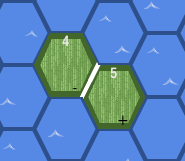
\includegraphics[width=5cm]{bridge_example.png}
\end{center}

Un panda peut se déplacer sur un même pont (à travers le trait blanc) sans contrainte. Pour passer d'un pont à l'autre, il faut que la hauteur du pont duquel le panda part soit la même que celle du pont sur lequel le panda veut aller. C'est le même fonctionnement que les dominos.

\begin{center}
    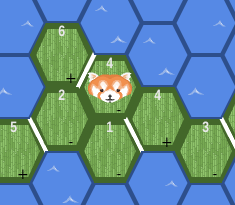
\includegraphics[width=6cm]{lots_of_bridges.png}
\end{center}

Lorsqu'un panda quitte une case d'un pont, la hauteur du pont change. Si c'était une case "+", la hauteur du pont augmente (plus 1 modulo 6). Si la case quittée était une case "-", la hauteur du pont diminue (moins 1 modulo 6). Les valeurs des cases de ponts sont donc toujours incluses entre 1 et 6.

\begin{center}
\begin{tabular}{c c}
     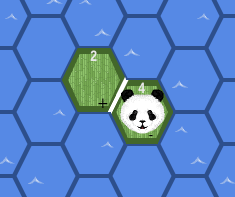
\includegraphics[height=5cm]{bridge_step_1.png} & 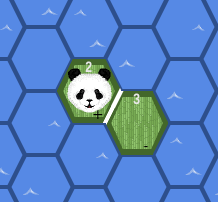
\includegraphics[height=5cm]{bridge_step_2.png} \\
\end{tabular}
\end{center}

\noindent Une fois quelques ponts construits, on peut obtenir ce genre de configuration :

\begin{center}
\begin{figure}[h]
    \centering
    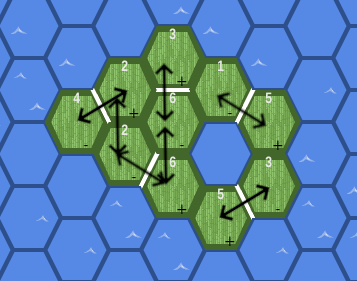
\includegraphics[width=6cm]{beaucoup_de_ponts_avec_fleches.png}
    \caption{Les flèches montrent les déplacements possibles}
\end{figure}
\end{center}

\subsubsection{Rochers}
Les rochers sont les obstacles naturels de la rivière. Rien ne peut traverser ni modifier une case de rocher.

\begin{center}
    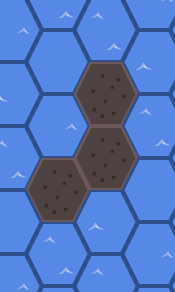
\includegraphics[width=4cm]{a_few_rocks.png}
\end{center}


\subsubsection{Pandas}
Les pandas sont ceux dont vous contrôlez le mouvement. Ils font toutes les actions sur la rivière. Ils peuvent poser des ponts, se déplacer et ramasser les bébés (cette dernière action est automatique). Il y les pandas géants (en noir et blanc), et les pandas roux (en blond vénitien). Ils sont toujours sur un pont.

\begin{center}
    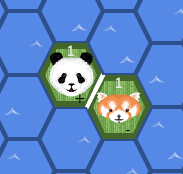
\includegraphics[width=6cm]{pandas_exemple.png}
\end{center}

\newpage

\subsubsection{Bébés pandas}
Les bébés pandas sont votre objectif ! C'est eux que vous devez sauver et qui vous feront gagner la partie. Ils sont toujours sur une case d'eau et ne peuvent pas se déplacer.

\begin{center}
    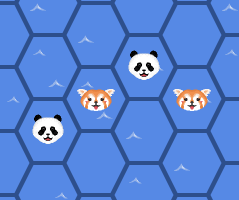
\includegraphics[width=6cm]{bebes_pandas_exemple.png}
\end{center}


\subsection{Déplacements}
Les pandas n'étant pas de grands amateurs des étendues d'eau\footnote{Ils savent bien nager, mais préfèrent éviter de mouiller leur magnifique pelage tout fluffy}, ils préfèrent se déplacer sur des ponts. Ils devront dont construire des ponts en bambou sur la rivière. C'est là qu'ils rencontreront la première grande difficulté : les fonds marins n'ont pas tous la même hauteur et sont très (très) sensibles. Le sable chinois au fond de la rivière de \textit{Hulun} se meut\footnote{Du verbe "mouvoir"} à la moindre perturbation. En plus de construire le pont, marcher dessus changera sa hauteur. Pouvoir passer d'un pont à l'autre pourrait ne plus être garanti à 100\% !

% insérer un screen d'une map avec uniquement des ponts sur l'eau

\section{Règles}
Revoyons ici les règles et modalités plus en détail. Vous êtes lancés sur une rivière constituée de cases hexagonales, deux pandas par joueurs. Les deux pandas sont les parents et se trouvent toujours forcément sur des ponts.

\subsection{Début d'une partie}
Au début, on place deux pandas par race à 4 endroits distincts ($p_1j_1$, $p_2j_1$, $p_1j_2$, $p_2j_2$)\footnote{p = panda, j = joueur}. Les bébés pandas et les ponts sont également placés, dépendamment de la carte chargée.

\subsection{Déroulement d'un tour}
L'ordre des tours est comme suit : panda 1 joueur 1, panda 1 joueur 2, panda 2 joueur 1, panda 2 joueur 2. Pour chaque panda, il est possible d'effectuer trois actions par tour :

\begin{itemize}
    \item Déplacement (ou non)
    \item Pose d'un pont (ou non)
    \item Déplacement (ou non)
\end{itemize}

\subsubsection{Pose d'un pont}
Pour poser un pont, il faut de la place. Vous ne pouvez pas poser un pont sur un bébé panda\footnote{Voir la section Bébés pandas pour comment ramasser un panda}, ni sur un autre pont. Vous ne pouvez pas poser un pont par-dessus un panda, car les pandas sont forcément sur un bout de pont. La valeur d'une case (ou sa hauteur) est uniquement modifiée lorsqu'un panda la \textit{quitte}.

% screen de ponts

\subsubsection{Déplacements}
Vous pouvez toujours vous déplacer d'un côté à l'autre d'un même pont. Ce qui sera la grande difficulté, c'est de passer d'un pont à l'autre. Les ponts ont tous des hauteurs et pour passer d'un pont à l'autre, il faut que la partie du pont sur laquelle vous êtes soit à la même hauteur que la partie du pont où vous voulez aller. Il n'y a pas de nombre de déplacements limités, mais vous ne pouvez pas revenir en arrière lors d'un déplacement atomique\footnote{déplacement atomique = déplacement d'une seule case. Vous pouvez en faire plusieurs, tant que c'est possible. Puis vous vous arrêtez.} !

% screen avec déplacements possibles et impossibles

\subsection{Les bébés pandas}
Les bébés pandas sont ce qui vous rapporte des points\footnote{Voir la partie "Points et Fin de partie"}. Le but est de ramasser tous les bébés. La répartition des bébés par parent panda n'est pas importante. Vous pouvez avoir un seul parent avec tous les bébés, comme les répartir sur les deux parents.

Pour ramasser un bébé panda, il suffit d'être sur une case adjacente. Le ramassage se fera automatiquement.

\subsection{Points et Fin de partie}
Une partie peut s'arrêter pour deux raisons :
\begin{itemize}
    \item une des races de panda a récupéré tous ses bébés
    \item la partie a atteint 200 tours
\end{itemize}

Le calcul se fait comme suit : lorsqu'un bébé panda est ramassé par un parent, il sera porté par ce parent jusqu'à la fin de la partie. Voici ce qu'on fait chaque tour\footnote{Un tour étant à la fin d'un cyce de 4 ponts posés et déplacements faits par les 4 parents pandas sur la map.} pour calculer les points du tour, qui seront additionnés aux points du joueur (classique). Pour chaque parent, on compte son nombre de bébés ramassés. Ce nombre est ensuite multiplié par 5. C'est le nombre de point que rapporte ce parent. Voici un exemple :

Disons qu'un parent panda géant porte un bébé depuis 2 tours et un autre bébé depuis 3 tours. Il aura rapporté au total 3 * 5 + 2 * 5 points depuis le début de la partie. Au tour suivant\footnote{Il faut attendre que les 3 autres aient joué leur tour}, il rapportera 10 points au total\footnote{A condition qu'il ne ramasse pas d'autre bébé pendant ce tour}, car il porte 2 bébés. Ce sont donc 2 * 5 = 10 points.



\newpage


\newpage
\section{API}
% This file was generated by stechec2-generator. DO NOT EDIT.

\noindent \begin{tabular}{lp{11cm}}
\textbf{Constante:} & NB\_TOURS \\
\textbf{Valeur:} & 200 \\
\textbf{Description:} & Nombre de tours à jouer avant la fin de la partie. \\
\end{tabular}
\vspace{0.2cm} \\

\noindent \begin{tabular}{lp{11cm}}
\textbf{Constante:} & NB\_PANDAS \\
\textbf{Valeur:} & 2 \\
\textbf{Description:} & Nombre de pandas par joueur. \\
\end{tabular}
\vspace{0.2cm} \\

\noindent \begin{tabular}{lp{11cm}}
\textbf{Constante:} & NB\_TOURS\_PERTE\_BEBE \\
\textbf{Valeur:} & 3 \\
\textbf{Description:} & Nombre de tours nécessaires pour faire tomber un bébé panda. \\
\end{tabular}
\vspace{0.2cm} \\

\noindent \begin{tabular}{lp{11cm}}
\textbf{Constante:} & VALEUR\_MAX\_PONT \\
\textbf{Valeur:} & 6 \\
\textbf{Description:} & Valeur max d'un pont (les valeurs sont comprises entre 1 et cette constante inclus). \\
\end{tabular}
\vspace{0.2cm} \\

\noindent \begin{tabular}{lp{11cm}}
\textbf{Constante:} & NB\_POINTS\_CAPTURE\_BEBE \\
\textbf{Valeur:} & 10 \\
\textbf{Description:} & Nombre de points obtenus à la capture d'un bébé pandas. \\
\end{tabular}
\vspace{0.2cm} \\


\functitle{case\_type} \\
\noindent
\begin{tabular}[t]{@{\extracolsep{0pt}}>{\bfseries}lp{10cm}}
Description~: & Types de cases \\
Valeurs~: &
\small
\begin{tabular}[t]{@{\extracolsep{0pt}}lp{7cm}}
    \textsl{LIBRE}~: & Case libre \\
    \textsl{OBSTACLE}~: & Obstacle \\
    \textsl{PONT}~: & Pont \\
    \textsl{BEBE}~: & Bébé panda \\
\end{tabular} \\
\end{tabular}

\functitle{direction} \\
\noindent
\begin{tabular}[t]{@{\extracolsep{0pt}}>{\bfseries}lp{10cm}}
Description~: & Directions cardinales \\
Valeurs~: &
\small
\begin{tabular}[t]{@{\extracolsep{0pt}}lp{7cm}}
    \textsl{NORD\_EST}~: & Direction : nord-est \\
    \textsl{SUD\_EST}~: & Direction : sud-est \\
    \textsl{SUD}~: & Direction : sud \\
    \textsl{SUD\_OUEST}~: & Direction : sud-ouest \\
    \textsl{NORD\_OUEST}~: & Direction : nord-ouest \\
    \textsl{NORD}~: & Direction : nord \\
\end{tabular} \\
\end{tabular}

\functitle{erreur} \\
\noindent
\begin{tabular}[t]{@{\extracolsep{0pt}}>{\bfseries}lp{10cm}}
Description~: & Erreurs possibles \\
Valeurs~: &
\small
\begin{tabular}[t]{@{\extracolsep{0pt}}lp{7cm}}
    \textsl{OK}~: & L'action s'est effectuée avec succès. \\
    \textsl{POSITION\_INVALIDE}~: & La position spécifiée n'est pas sur la rivière. \\
    \textsl{POSITION\_OBSTACLE}~: & La position spécifiée est un obstacle. \\
    \textsl{MAUVAIS\_NOMBRE}~: & La hauteur de la position spécifiée ne correspond pas. \\
    \textsl{DEPLACEMENT\_HORS\_LIMITES}~: & Ce déplacement fait sortir un panda des limites de la rivière. \\
    \textsl{DIRECTION\_INVALIDE}~: & La direction spécifiée n'existe pas. \\
    \textsl{MOUVEMENT\_INVALIDE}~: & Le panda ne peut pas se déplacer dans cette direction. \\
    \textsl{POSE\_INVALIDE}~: & Le pont ne peut pas être placé a cette position et dans cette direction. \\
    \textsl{ID\_PANDA\_INVALIDE}~: & Le panda spécifié n'existe pas. \\
    \textsl{ACTION\_DEJA\_EFFECTUEE}~: & Une action a déjà été effectuée ce tour. \\
    \textsl{DRAPEAU\_INVALIDE}~: & Le drapeau spécifié n'existe pas. \\
    \textsl{DEPLACEMENT\_EN\_ARRIERE}~: & La panda c'est déjà déplacé sur cette case. \\
\end{tabular} \\
\end{tabular}

\functitle{action\_type} \\
\noindent
\begin{tabular}[t]{@{\extracolsep{0pt}}>{\bfseries}lp{10cm}}
Description~: & Types d'actions \\
Valeurs~: &
\small
\begin{tabular}[t]{@{\extracolsep{0pt}}lp{7cm}}
    \textsl{ACTION\_DEPLACER}~: & Action ``deplacer``. \\
    \textsl{ACTION\_POSER}~: & Action ``poser``. \\
\end{tabular} \\
\end{tabular}

\functitle{debug\_drapeau} \\
\noindent
\begin{tabular}[t]{@{\extracolsep{0pt}}>{\bfseries}lp{10cm}}
Description~: & Types de drapeau de débug \\
Valeurs~: &
\small
\begin{tabular}[t]{@{\extracolsep{0pt}}lp{7cm}}
    \textsl{AUCUN\_DRAPEAU}~: & Aucun drapeau, enlève le drapeau présent \\
    \textsl{DRAPEAU\_BLEU}~: & Drapeau bleu \\
    \textsl{DRAPEAU\_VERT}~: & Drapeau vert \\
    \textsl{DRAPEAU\_ROUGE}~: & Drapeau rouge \\
\end{tabular} \\
\end{tabular}



\functitle{position}
\begin{lst-c++}
struct position {
    int x;
    int y;
};
\end{lst-c++}
\noindent
\begin{tabular}[t]{@{\extracolsep{0pt}}>{\bfseries}lp{10cm}}
Description~: & Position du panda. \\
Champs~: &
\small
\begin{tabular}[t]{@{\extracolsep{0pt}}lp{7cm}}
    \textsl{x}~: & Coordonnée : x \\
    \textsl{y}~: & Coordonnée : y \\
\end{tabular} \\
\end{tabular}

\functitle{pont\_type}
\begin{lst-c++}
struct pont\_type {
    position debut_pos;
    position fin_pos;
    int debut_val;
    int fin_val;
};
\end{lst-c++}
\noindent
\begin{tabular}[t]{@{\extracolsep{0pt}}>{\bfseries}lp{10cm}}
Description~: & Case type pont, contient la case de début et de fin. La case de début a une valeur qui s'incrémente, et celle de fin se decrémente. \\
Champs~: &
\small
\begin{tabular}[t]{@{\extracolsep{0pt}}lp{7cm}}
    \textsl{debut\_pos}~: & Position de la case de début \\
    \textsl{fin\_pos}~: & Position de la case de fin \\
    \textsl{debut\_val}~: & Valeur de la case de début \\
    \textsl{fin\_val}~: & Valeur de la case de début \\
\end{tabular} \\
\end{tabular}

\functitle{panda\_info}
\begin{lst-c++}
struct panda\_info {
    position panda_pos;
    int id_joueur;
    int id_panda;
    int num_bebes;
};
\end{lst-c++}
\noindent
\begin{tabular}[t]{@{\extracolsep{0pt}}>{\bfseries}lp{10cm}}
Description~: & Panda et son joueur \\
Champs~: &
\small
\begin{tabular}[t]{@{\extracolsep{0pt}}lp{7cm}}
    \textsl{panda\_pos}~: & Position du panda \\
    \textsl{id\_joueur}~: & Identifiant du joueur qui contrôle le panda \\
    \textsl{id\_panda}~: & Identifiant du panda relatif au joueur \\
    \textsl{num\_bebes}~: & Nombre de bébés qui sont portés par le panda parent \\
\end{tabular} \\
\end{tabular}

\functitle{bebe\_info}
\begin{lst-c++}
struct bebe\_info {
    position bebe_pos;
    int id_bebe_joueur;
};
\end{lst-c++}
\noindent
\begin{tabular}[t]{@{\extracolsep{0pt}}>{\bfseries}lp{10cm}}
Description~: & Bébé panda à ramener. \\
Champs~: &
\small
\begin{tabular}[t]{@{\extracolsep{0pt}}lp{7cm}}
    \textsl{bebe\_pos}~: & Position du bébé panda \\
    \textsl{id\_bebe\_joueur}~: & Identifiant du joueur qui peut saver le bébé \\
\end{tabular} \\
\end{tabular}

\functitle{tour\_info}
\begin{lst-c++}
struct tour\_info {
    int id_panda_joue;
    int id_tour;
};
\end{lst-c++}
\noindent
\begin{tabular}[t]{@{\extracolsep{0pt}}>{\bfseries}lp{10cm}}
Description~: & Information sur un tour particulier. \\
Champs~: &
\small
\begin{tabular}[t]{@{\extracolsep{0pt}}lp{7cm}}
    \textsl{id\_panda\_joue}~: & Identifiant du panda qui joue \\
    \textsl{id\_tour}~: & Identifiant unique du tour (compteur) \\
\end{tabular} \\
\end{tabular}

\functitle{carte\_info}
\begin{lst-c++}
struct carte\_info {
    int taille_x;
    int taille_y;
};
\end{lst-c++}
\noindent
\begin{tabular}[t]{@{\extracolsep{0pt}}>{\bfseries}lp{10cm}}
Description~: & Information sur la carte de la partie en cours. \\
Champs~: &
\small
\begin{tabular}[t]{@{\extracolsep{0pt}}lp{7cm}}
    \textsl{taille\_x}~: & La taille de la carte pour les coordonnées x {[}0; taille\_x{[} \\
    \textsl{taille\_y}~: & La taille de la carte pour les coordonnées y {[}0; taille\_y{[} \\
\end{tabular} \\
\end{tabular}

\functitle{action\_hist}
\begin{lst-c++}
struct action\_hist {
    action_type type_action;
    int action_id_panda;
    direction dir;
    int valeur_debut;
    int valeur_fin;
    position pos_debut;
    position pos_fin;
};
\end{lst-c++}
\noindent
\begin{tabular}[t]{@{\extracolsep{0pt}}>{\bfseries}lp{10cm}}
Description~: & Action représentée dans l'historique. \\
Champs~: &
\small
\begin{tabular}[t]{@{\extracolsep{0pt}}lp{7cm}}
    \textsl{type\_action}~: & Type de l'action \\
    \textsl{action\_id\_panda}~: & Identifiant du panda concerné par l'action \\
    \textsl{dir}~: & Direction visée par le panda durant le déplacement \\
    \textsl{valeur\_debut}~: & Valeur au début du pont posé (de 1 à 6 inclus) \\
    \textsl{valeur\_fin}~: & Valeur à la fin du pont posé (de 1 à 6 inclus) \\
    \textsl{pos\_debut}~: & Position du début du pont posé \\
    \textsl{pos\_fin}~: & Position de la fin du pont posé \\
\end{tabular} \\
\end{tabular}



\begin{minipage}{\linewidth}
\functitle{deplacer}
\begin{lst-c++}
erreur deplacer(direction dir)
\end{lst-c++}
\noindent
\begin{tabular}[t]{@{\extracolsep{0pt}}>{\bfseries}lp{10cm}}
Description~: & Déplace le panda ``id\_panda`` sur le pont choisi. \\
Paramètres~: &
\begin{tabular}[t]{@{\extracolsep{0pt}}ll}
    \textsl{dir}~: & Direction visée \\
  \end{tabular} \\
\end{tabular} \\[0.3cm]
\end{minipage}

\begin{minipage}{\linewidth}
\functitle{poser}
\begin{lst-c++}
erreur poser(position position_debut, direction dir, int pont_debut, int pont_fin)
\end{lst-c++}
\noindent
\begin{tabular}[t]{@{\extracolsep{0pt}}>{\bfseries}lp{10cm}}
Description~: & Pose un pont dans la direction choisie à partir du panda ``id\_panda``. \\
Paramètres~: &
\begin{tabular}[t]{@{\extracolsep{0pt}}ll}
    \textsl{position\_debut}~: & Position de début du pont \\
    \textsl{dir}~: & Direction visée \\
    \textsl{pont\_debut}~: & Début du pont placé \\
    \textsl{pont\_fin}~: & Fin du pont \\
  \end{tabular} \\
\end{tabular} \\[0.3cm]
\end{minipage}

\begin{minipage}{\linewidth}
\functitle{debug\_afficher\_drapeau}
\begin{lst-c++}
erreur debug_afficher_drapeau(position pos, debug_drapeau drapeau)
\end{lst-c++}
\noindent
\begin{tabular}[t]{@{\extracolsep{0pt}}>{\bfseries}lp{10cm}}
Description~: & Affiche le drapeau spécifié sur la case indiquée \\
Paramètres~: &
\begin{tabular}[t]{@{\extracolsep{0pt}}ll}
    \textsl{pos}~: & Case ciblée \\
    \textsl{drapeau}~: & Drapeau à afficher sur la case \\
  \end{tabular} \\
\end{tabular} \\[0.3cm]
\end{minipage}

\begin{minipage}{\linewidth}
\functitle{type\_case}
\begin{lst-c++}
case_type type_case(position pos)
\end{lst-c++}
\noindent
\begin{tabular}[t]{@{\extracolsep{0pt}}>{\bfseries}lp{10cm}}
Description~: & Renvoie le type d'une case donnée. \\
Paramètres~: &
\begin{tabular}[t]{@{\extracolsep{0pt}}ll}
    \textsl{pos}~: & Case choisie \\
  \end{tabular} \\
\end{tabular} \\[0.3cm]
\end{minipage}

\begin{minipage}{\linewidth}
\functitle{panda\_sur\_case}
\begin{lst-c++}
int panda_sur_case(position pos)
\end{lst-c++}
\noindent
\begin{tabular}[t]{@{\extracolsep{0pt}}>{\bfseries}lp{10cm}}
Description~: & Renvoie le numéro du joueur à qui appartient panda sur la case indiquée. Renvoie -1 s'il n'y a pas de panda ou si la position est invalide. \\
Paramètres~: &
\begin{tabular}[t]{@{\extracolsep{0pt}}ll}
    \textsl{pos}~: & Case choisie \\
  \end{tabular} \\
\end{tabular} \\[0.3cm]
\end{minipage}

\begin{minipage}{\linewidth}
\functitle{bebe\_panda\_sur\_case}
\begin{lst-c++}
int bebe_panda_sur_case(position pos)
\end{lst-c++}
\noindent
\begin{tabular}[t]{@{\extracolsep{0pt}}>{\bfseries}lp{10cm}}
Description~: & Renvoie le numéro du joueur à qui appartient le bébé panda sur la case indiquée. Renvoie -1 s'il n'y a pas de bébé panda ou si la position est invalide. \\
Paramètres~: &
\begin{tabular}[t]{@{\extracolsep{0pt}}ll}
    \textsl{pos}~: & Case choisie \\
  \end{tabular} \\
\end{tabular} \\[0.3cm]
\end{minipage}

\begin{minipage}{\linewidth}
\functitle{position\_panda}
\begin{lst-c++}
position position_panda(int id_joueur, int id_panda)
\end{lst-c++}
\noindent
\begin{tabular}[t]{@{\extracolsep{0pt}}>{\bfseries}lp{10cm}}
Description~: & Indique la position du panda sur la rivière désigné par le numéro ``id\_panda`` appartenant au joueur ``id\_joueur``. Si la description du panda est incorrecte, la position (-1, -1) est renvoyée. \\
Paramètres~: &
\begin{tabular}[t]{@{\extracolsep{0pt}}ll}
    \textsl{id\_joueur}~: & Numéro du joueur \\
    \textsl{id\_panda}~: & Numéro du panda \\
  \end{tabular} \\
\end{tabular} \\[0.3cm]
\end{minipage}

\begin{minipage}{\linewidth}
\functitle{info\_pont}
\begin{lst-c++}
pont_type info_pont(position pos)
\end{lst-c++}
\noindent
\begin{tabular}[t]{@{\extracolsep{0pt}}>{\bfseries}lp{10cm}}
Description~: & Renvoie les informations relatives au pont situé à cette position. Le pont est constitué de deux cases. Si aucun pont n'est placé à cette position ou si la position est invalide, les membres debut\_val et fin\_val de la structure ``pont\_type`` renvoyée sont initialisés à -1. \\
Paramètres~: &
\begin{tabular}[t]{@{\extracolsep{0pt}}ll}
    \textsl{pos}~: & Case choisie \\
  \end{tabular} \\
\end{tabular} \\[0.3cm]
\end{minipage}

\begin{minipage}{\linewidth}
\functitle{info\_panda}
\begin{lst-c++}
panda_info info_panda(position pos)
\end{lst-c++}
\noindent
\begin{tabular}[t]{@{\extracolsep{0pt}}>{\bfseries}lp{10cm}}
Description~: & Renvoie la description d'un panda en fonction d'une position donnée. Si le panda n'est pas présent sur la carte, ou si la position est invalide, tous les membres de la structure ``panda\_info`` renvoyée sont initialisés à -1. \\
Paramètres~: &
\begin{tabular}[t]{@{\extracolsep{0pt}}ll}
    \textsl{pos}~: & Case choisie \\
  \end{tabular} \\
\end{tabular} \\[0.3cm]
\end{minipage}

\begin{minipage}{\linewidth}
\functitle{liste\_pandas}
\begin{lst-c++}
panda_info array liste_pandas()
\end{lst-c++}
\noindent
\begin{tabular}[t]{@{\extracolsep{0pt}}>{\bfseries}lp{10cm}}
Description~: & Renvoie la liste de tous les pandas présents durant la partie. \\
\end{tabular} \\[0.3cm]
\end{minipage}

\begin{minipage}{\linewidth}
\functitle{liste\_bebes}
\begin{lst-c++}
bebe_info array liste_bebes()
\end{lst-c++}
\noindent
\begin{tabular}[t]{@{\extracolsep{0pt}}>{\bfseries}lp{10cm}}
Description~: & Renvoie la liste de tous les bébés présents sur la carte, et et pas encore sauvés. \\
\end{tabular} \\[0.3cm]
\end{minipage}

\begin{minipage}{\linewidth}
\functitle{positions\_adjacentes}
\begin{lst-c++}
position array positions_adjacentes(position pos)
\end{lst-c++}
\noindent
\begin{tabular}[t]{@{\extracolsep{0pt}}>{\bfseries}lp{10cm}}
Description~: & Renvoie la liste de toutes les positions adjacentes à la position donnée. \\
Paramètres~: &
\begin{tabular}[t]{@{\extracolsep{0pt}}ll}
    \textsl{pos}~: & Case choisie \\
  \end{tabular} \\
\end{tabular} \\[0.3cm]
\end{minipage}

\begin{minipage}{\linewidth}
\functitle{position\_dans\_direction}
\begin{lst-c++}
position position_dans_direction(position pos, direction dir)
\end{lst-c++}
\noindent
\begin{tabular}[t]{@{\extracolsep{0pt}}>{\bfseries}lp{10cm}}
Description~: & Renvoie la position relative à la direction donnée par rapport à une position d'origine. Si une telle position serait invalide, la position \{-1, -1\} est renvoyée. \\
Paramètres~: &
\begin{tabular}[t]{@{\extracolsep{0pt}}ll}
    \textsl{pos}~: & Position d'origine \\
    \textsl{dir}~: & Direction \\
  \end{tabular} \\
\end{tabular} \\[0.3cm]
\end{minipage}

\begin{minipage}{\linewidth}
\functitle{direction\_entre\_positions}
\begin{lst-c++}
int direction_entre_positions(position origine, position cible)
\end{lst-c++}
\noindent
\begin{tabular}[t]{@{\extracolsep{0pt}}>{\bfseries}lp{10cm}}
Description~: & Renvoie la direction telle que position\_dans\_direction(origine, cible) == direction. Si aucune telle direction n'existe, -1 est renvoyée. \\
Paramètres~: &
\begin{tabular}[t]{@{\extracolsep{0pt}}ll}
    \textsl{origine}~: & Position d'origine \\
    \textsl{cible}~: & Position relative à l'origine \\
  \end{tabular} \\
\end{tabular} \\[0.3cm]
\end{minipage}

\begin{minipage}{\linewidth}
\functitle{historique}
\begin{lst-c++}
action_hist array historique()
\end{lst-c++}
\noindent
\begin{tabular}[t]{@{\extracolsep{0pt}}>{\bfseries}lp{10cm}}
Description~: & Renvoie la liste des actions effectuées par l’adversaire durant son tour, dans l'ordre chronologique. Les actions de débug n'apparaissent pas dans cette liste. \\
\end{tabular} \\[0.3cm]
\end{minipage}

\begin{minipage}{\linewidth}
\functitle{score}
\begin{lst-c++}
int score(int id_joueur)
\end{lst-c++}
\noindent
\begin{tabular}[t]{@{\extracolsep{0pt}}>{\bfseries}lp{10cm}}
Description~: & Renvoie le score du joueur ``id\_joueur``. Renvoie -1 si le joueur est invalide. \\
Paramètres~: &
\begin{tabular}[t]{@{\extracolsep{0pt}}ll}
    \textsl{id\_joueur}~: & Numéro du joueur \\
  \end{tabular} \\
\end{tabular} \\[0.3cm]
\end{minipage}

\begin{minipage}{\linewidth}
\functitle{moi}
\begin{lst-c++}
int moi()
\end{lst-c++}
\noindent
\begin{tabular}[t]{@{\extracolsep{0pt}}>{\bfseries}lp{10cm}}
Description~: & Renvoie votre numéro de joueur. \\
\end{tabular} \\[0.3cm]
\end{minipage}

\begin{minipage}{\linewidth}
\functitle{adversaire}
\begin{lst-c++}
int adversaire()
\end{lst-c++}
\noindent
\begin{tabular}[t]{@{\extracolsep{0pt}}>{\bfseries}lp{10cm}}
Description~: & Renvoie le numéro de joueur de votre adversaire. \\
\end{tabular} \\[0.3cm]
\end{minipage}

\begin{minipage}{\linewidth}
\functitle{info\_tour}
\begin{lst-c++}
tour_info info_tour()
\end{lst-c++}
\noindent
\begin{tabular}[t]{@{\extracolsep{0pt}}>{\bfseries}lp{10cm}}
Description~: & Renvoie le tour actuel. \\
\end{tabular} \\[0.3cm]
\end{minipage}

\begin{minipage}{\linewidth}
\functitle{info\_carte}
\begin{lst-c++}
carte_info info_carte()
\end{lst-c++}
\noindent
\begin{tabular}[t]{@{\extracolsep{0pt}}>{\bfseries}lp{10cm}}
Description~: & Renvoie la carte pour la partie en cours. \\
\end{tabular} \\[0.3cm]
\end{minipage}

\begin{minipage}{\linewidth}
\functitle{afficher\_case\_type}
\begin{lst-c++}
void afficher_case_type(case_type v)
\end{lst-c++}
\noindent
\begin{tabular}[t]{@{\extracolsep{0pt}}>{\bfseries}lp{10cm}}
Description~: & Affiche le contenu d'une valeur de type case\_type \\
Paramètres~: &
\begin{tabular}[t]{@{\extracolsep{0pt}}ll}
    \textsl{v}~: & The value to display \\
  \end{tabular} \\
\end{tabular} \\[0.3cm]
\end{minipage}

\begin{minipage}{\linewidth}
\functitle{afficher\_direction}
\begin{lst-c++}
void afficher_direction(direction v)
\end{lst-c++}
\noindent
\begin{tabular}[t]{@{\extracolsep{0pt}}>{\bfseries}lp{10cm}}
Description~: & Affiche le contenu d'une valeur de type direction \\
Paramètres~: &
\begin{tabular}[t]{@{\extracolsep{0pt}}ll}
    \textsl{v}~: & The value to display \\
  \end{tabular} \\
\end{tabular} \\[0.3cm]
\end{minipage}

\begin{minipage}{\linewidth}
\functitle{afficher\_erreur}
\begin{lst-c++}
void afficher_erreur(erreur v)
\end{lst-c++}
\noindent
\begin{tabular}[t]{@{\extracolsep{0pt}}>{\bfseries}lp{10cm}}
Description~: & Affiche le contenu d'une valeur de type erreur \\
Paramètres~: &
\begin{tabular}[t]{@{\extracolsep{0pt}}ll}
    \textsl{v}~: & The value to display \\
  \end{tabular} \\
\end{tabular} \\[0.3cm]
\end{minipage}

\begin{minipage}{\linewidth}
\functitle{afficher\_action\_type}
\begin{lst-c++}
void afficher_action_type(action_type v)
\end{lst-c++}
\noindent
\begin{tabular}[t]{@{\extracolsep{0pt}}>{\bfseries}lp{10cm}}
Description~: & Affiche le contenu d'une valeur de type action\_type \\
Paramètres~: &
\begin{tabular}[t]{@{\extracolsep{0pt}}ll}
    \textsl{v}~: & The value to display \\
  \end{tabular} \\
\end{tabular} \\[0.3cm]
\end{minipage}

\begin{minipage}{\linewidth}
\functitle{afficher\_debug\_drapeau}
\begin{lst-c++}
void afficher_debug_drapeau(debug_drapeau v)
\end{lst-c++}
\noindent
\begin{tabular}[t]{@{\extracolsep{0pt}}>{\bfseries}lp{10cm}}
Description~: & Affiche le contenu d'une valeur de type debug\_drapeau \\
Paramètres~: &
\begin{tabular}[t]{@{\extracolsep{0pt}}ll}
    \textsl{v}~: & The value to display \\
  \end{tabular} \\
\end{tabular} \\[0.3cm]
\end{minipage}

\begin{minipage}{\linewidth}
\functitle{afficher\_position}
\begin{lst-c++}
void afficher_position(position v)
\end{lst-c++}
\noindent
\begin{tabular}[t]{@{\extracolsep{0pt}}>{\bfseries}lp{10cm}}
Description~: & Affiche le contenu d'une valeur de type position \\
Paramètres~: &
\begin{tabular}[t]{@{\extracolsep{0pt}}ll}
    \textsl{v}~: & The value to display \\
  \end{tabular} \\
\end{tabular} \\[0.3cm]
\end{minipage}

\begin{minipage}{\linewidth}
\functitle{afficher\_pont\_type}
\begin{lst-c++}
void afficher_pont_type(pont_type v)
\end{lst-c++}
\noindent
\begin{tabular}[t]{@{\extracolsep{0pt}}>{\bfseries}lp{10cm}}
Description~: & Affiche le contenu d'une valeur de type pont\_type \\
Paramètres~: &
\begin{tabular}[t]{@{\extracolsep{0pt}}ll}
    \textsl{v}~: & The value to display \\
  \end{tabular} \\
\end{tabular} \\[0.3cm]
\end{minipage}

\begin{minipage}{\linewidth}
\functitle{afficher\_panda\_info}
\begin{lst-c++}
void afficher_panda_info(panda_info v)
\end{lst-c++}
\noindent
\begin{tabular}[t]{@{\extracolsep{0pt}}>{\bfseries}lp{10cm}}
Description~: & Affiche le contenu d'une valeur de type panda\_info \\
Paramètres~: &
\begin{tabular}[t]{@{\extracolsep{0pt}}ll}
    \textsl{v}~: & The value to display \\
  \end{tabular} \\
\end{tabular} \\[0.3cm]
\end{minipage}

\begin{minipage}{\linewidth}
\functitle{afficher\_bebe\_info}
\begin{lst-c++}
void afficher_bebe_info(bebe_info v)
\end{lst-c++}
\noindent
\begin{tabular}[t]{@{\extracolsep{0pt}}>{\bfseries}lp{10cm}}
Description~: & Affiche le contenu d'une valeur de type bebe\_info \\
Paramètres~: &
\begin{tabular}[t]{@{\extracolsep{0pt}}ll}
    \textsl{v}~: & The value to display \\
  \end{tabular} \\
\end{tabular} \\[0.3cm]
\end{minipage}

\begin{minipage}{\linewidth}
\functitle{afficher\_tour\_info}
\begin{lst-c++}
void afficher_tour_info(tour_info v)
\end{lst-c++}
\noindent
\begin{tabular}[t]{@{\extracolsep{0pt}}>{\bfseries}lp{10cm}}
Description~: & Affiche le contenu d'une valeur de type tour\_info \\
Paramètres~: &
\begin{tabular}[t]{@{\extracolsep{0pt}}ll}
    \textsl{v}~: & The value to display \\
  \end{tabular} \\
\end{tabular} \\[0.3cm]
\end{minipage}

\begin{minipage}{\linewidth}
\functitle{afficher\_carte\_info}
\begin{lst-c++}
void afficher_carte_info(carte_info v)
\end{lst-c++}
\noindent
\begin{tabular}[t]{@{\extracolsep{0pt}}>{\bfseries}lp{10cm}}
Description~: & Affiche le contenu d'une valeur de type carte\_info \\
Paramètres~: &
\begin{tabular}[t]{@{\extracolsep{0pt}}ll}
    \textsl{v}~: & The value to display \\
  \end{tabular} \\
\end{tabular} \\[0.3cm]
\end{minipage}

\begin{minipage}{\linewidth}
\functitle{afficher\_action\_hist}
\begin{lst-c++}
void afficher_action_hist(action_hist v)
\end{lst-c++}
\noindent
\begin{tabular}[t]{@{\extracolsep{0pt}}>{\bfseries}lp{10cm}}
Description~: & Affiche le contenu d'une valeur de type action\_hist \\
Paramètres~: &
\begin{tabular}[t]{@{\extracolsep{0pt}}ll}
    \textsl{v}~: & The value to display \\
  \end{tabular} \\
\end{tabular} \\[0.3cm]
\end{minipage}

\newpage
\section{Notes sur l'utilisation de l'API}
\subsection{C}

\begin{itemize}
\item{Les booléens sont représentés par le type \texttt{bool}, défini par le
      standard du C99, et que l'on retrouve dans le header \texttt{stdbool.h};}
\item{Les fonctions prenant des tableaux en paramètres et retournant des
      tableaux utilisent à la place de ces tableaux une structure
      \texttt{type\_array}, où \texttt{type} est le type des données dans le
      tableau. Ces structures contiennent deux éléments : les données,
      \texttt{type* items}, et la taille, \texttt{size\_t length}. Dans tous les
      cas, la libération des données est laissée au soin du candidat ;}
\item{Tout le reste est comme indiqué dans le sujet.}
\end{itemize}

\subsection{C++}

\begin{itemize}
\item{Les tableaux sont représentés par des \texttt{std::vector<type>} ;}
\item{Le reste est identique au sujet.}
\end{itemize}

\subsection{C\#}

\begin{itemize}
\item{Les fonctions à utiliser sont des méthodes statiques de la classe
      \texttt{Api}.
      Ainsi, pour utiliser la fonction \texttt{Foo}, il faut faire
      \texttt{Api.Foo} ;}
\item{Les noms des fonctions, structures et énumérations sont en
      \texttt{CamelCase}. Ainsi, une fonction nommée \texttt{foo\_bar} dans
      le sujet s'appellera \texttt{FooBar} en C\#.}
\end{itemize}

\subsection{Haskell}

\begin{itemize}
\item{L'API est fournie par le module \texttt{Api}.}
\item{Les énumérations sont représentées par des types sommes, les structures
      par des records. Seule la première lettre des noms de types et de
      constructeurs est en majuscule. Le nom du constructeur d'une structure
      est son nom de type.}
\item{La commande \texttt{make doc} permet de générer la documentation dans le
      fichier \texttt{doc/index.html} pour votre code ainsi que pour l'API.}
\item{Pour pouvoir conserver des valeurs entre différents appels à vos fonctions
      à compléter, il faut utiliser des variables mutables :}
\begin{lstlisting}[language=Haskell]
import Data.IORef
import System.IO.Unsafe (unsafePerformIO)

-- La pragma NOINLINE est importante !
-- MonType ne doit pas etre polymorphe !
{-# NOINLINE maVariable #-}
maVariable :: IORef MonType
maVariable = unsafePerformIO (newIORef maValeurInitiale)

fonctionACompleter :: IO ()
fonctionACompleter = do
  maValeur <- readIORef maVariable
  ...
  writeIORef maVariable maValeur'

\end{lstlisting}
\end{itemize}

\subsection{Java}

\begin{itemize}
\item{Les fonctions à utiliser sont des méthodes statiques de la classe
      \texttt{Interface}. Ainsi, pour utiliser la fonction \texttt{foo}, il
      faut faire \texttt{Interface.foo} ;}
\item{Les structures sont représentées par des classes dont tous les attributs
      sont publics.}
\end{itemize}

\subsection{OCaml}

\begin{itemize}
\item{L'API est fournie par le fichier \texttt{api.ml}, qui est \texttt{open}
      par défaut par le fichier à compléter ;}
\item{Les énumérations sont représentées par des types sommes avec des
      constructeurs sans paramètres. Seule la première lettre des noms des
      constructeurs est en majuscule ;}

\item{Les structures sont représentées par des records, sauf pour la structure
      \texttt{position} qui est représentée par un couple \texttt{int * int} ;}
\item{Les tableaux sont représentés par des \texttt{array} Caml classiques.}
\end{itemize}

\subsection{PHP}

\begin{itemize}
\item{Les constantes sont définies via des \texttt{define} et doivent donc être
      utilisées sans les précéder d'un signe dollar ;}
\item{Les énumérations sont définies comme des séries de constantes. Se référer
      à la puce au-dessus ;}
\item{Les structures sont gérées sous forme de tableaux associatifs. Ainsi, une
      structure contenant un champ \texttt{x} et un champ \texttt{y} sera créée
      comme ceci : \texttt{array('x' => 42, 'y' => 1337)}.}
\end{itemize}

\subsection{Python}

\begin{itemize}
\item{L'API est fournie par le module \texttt{api}, dont tout le contenu est
      importé par défaut par le code à compléter ;}
\item{Les énumérations sont représentées par des \texttt{IntEnum} Python, qui
      peuvent être utilisées comme ceci : \texttt{nom\_enum.CHAMP}. ;}
\item{Les structures sont représentées par des \texttt{NamedTuple} Python, dont
      on peut accéder aux champs via la notation pointée habituelle, et
      qui peuvent être créés comme ceci : \texttt{foo(bar=42, x=3)}, sauf pour
      la structure \texttt{position} qui est représentée par un couple (x, y).}
\end{itemize}

\subsection{Rust}

\begin{itemize}
\item{L'API est fournie par le module \texttt{api}, dont tout le contenu est
      importé par défaut par le code à compléter. ;}
\item{Les noms des structures et énumérations sont en \texttt{CamelCase}.
      Ainsi, une structure nommée \texttt{foo\_bar} dans le sujet
      s'appellera \texttt{FooBar} en Rust.}
\item{Les tableaux sont représentés par des \texttt{Vec<T>} et les strings par
      des \texttt{String}. Les fonctions prennent leurs primitives empruntées
      \texttt{\&[T]} et \texttt{\&str} en entrée.}
\end{itemize}


\clearpage
\vspace*{\fill}
\begin{center}
\begin{minipage}{.5\textwidth}
Bonne chance !
\end{minipage}
\end{center}
\vfill % equivalent to \vspace{\fill}
\clearpage


\end{document}
